% Figure: the four-way splits. (a) charts near a base line in the (delta, t) plane at a fixed tilt u;
% (b) the zones around a corner point of a face; (c) wedge-corner zones and the ray zones.
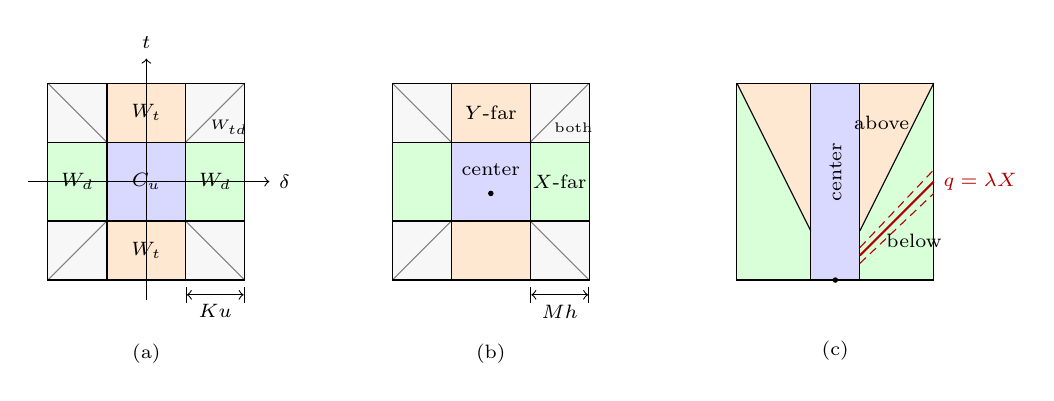
\begin{tikzpicture}[font=\scriptsize,x=1.25cm,y=1.25cm]
 \def\ttfourway{%
  \fill[gray!6] (-1,-1) rectangle (1,1);
  \fill[blue!15] (-0.4,-0.4) rectangle (0.4,0.4);
  \fill[orange!18] (-0.4,0.4) rectangle (0.4,1); \fill[orange!18] (-0.4,-1) rectangle (0.4,-0.4);
  \fill[green!15] (0.4,-0.4) rectangle (1,0.4); \fill[green!15] (-1,-0.4) rectangle (-0.4,0.4);
  \foreach \sx in {1,-1} \foreach \sy in {1,-1} \draw[gray] (0.4*\sx,0.4*\sy) -- (\sx,\sy);
  \draw (-1,-1) rectangle (1,1); \draw (-0.4,-1) -- (-0.4,1) (0.4,-1) -- (0.4,1) (-1,-0.4) -- (1,-0.4) (-1,0.4) -- (1,0.4);}
 \begin{scope}
  \ttfourway
  \node at (0,0) {$C_u$}; \node at (0,0.7) {$W_t$}; \node at (0,-0.7) {$W_t$}; \node at (0.7,0) {$W_d$}; \node at (-0.7,0) {$W_d$};
  \node[font=\tiny] at (0.84,0.55) {$W_{td}$};
  \draw[->] (-1.2,0) -- (1.25,0) node[right] {$\delta$}; \draw[->] (0,-1.2) -- (0,1.25) node[above] {$t$};
  \draw[|<->|] (0.4,-1.15) -- node[below] {$Ku$} (1,-1.15);
  \node at (0,-1.75) {(a)};
 \end{scope}
 \begin{scope}[shift={(3.5,0)}]
  \ttfourway
  \node at (0,0.12) {center}; \node at (0,0.7) {$Y$-far}; \node at (0.7,0) {$X$-far}; \node[font=\tiny] at (0.84,0.55) {both};
  \fill (0,-0.12) circle (1pt);
  \draw[|<->|] (0.4,-1.15) -- node[below] {$Mh$} (1,-1.15);
  \node at (0,-1.75) {(b)};
 \end{scope}
 \begin{scope}[shift={(7.0,-1)},y=2.5cm]
  \fill[gray!6] (-1,0) rectangle (1,1);
  \fill[blue!15] (-0.25,0) rectangle (0.25,1);
  \fill[green!15] (0.25,0) -- (1,0) -- (1,1) -- (0.25,0.25) -- cycle; \fill[green!15] (-0.25,0) -- (-1,0) -- (-1,1) -- (-0.25,0.25) -- cycle;
  \fill[orange!18] (0.25,0.25) -- (1,1) -- (0.25,1) -- cycle; \fill[orange!18] (-0.25,0.25) -- (-1,1) -- (-0.25,1) -- cycle;
  \draw (-1,0) rectangle (1,1); \draw (-0.25,0) -- (-0.25,1) (0.25,0) -- (0.25,1);
  \draw (0.25,0.25) -- (1,1) (-0.25,0.25) -- (-1,1);
  \draw[red!70!black,thick] (0.25,0.125) -- (1,0.5);
  \draw[red!70!black,densely dashed] (0.25,0.085) -- (1,0.44) (0.25,0.165) -- (1,0.56);
  \node[rotate=90] at (0,0.55) {center};
  \node at (0.47,0.8) {above}; \node at (0.8,0.2) {below};
  \node[red!70!black,right] at (1,0.5) {$q=\lambda X$};
  \fill (0,0) circle (1pt);
  \node at (0,-0.36) {(c)};
 \end{scope}
\end{tikzpicture}
